\documentclass{article}
\usepackage{fullpage}
%%%%%%%%%%%%%%%%%%%%%%%%%%%%%%%%%%%
\usepackage{graphicx}
\usepackage{epstopdf}
\usepackage{amsthm}
\usepackage{amsmath}
\usepackage{amssymb}
\usepackage{caption}
\usepackage{subcaption}
\usepackage[all]{xy}



\everymath{\displaystyle}

\newenvironment{solution}
  {\begin{proof}[Solution]}
  {\end{proof}}
\newtheorem{definition}{Definition}
\newtheorem{example}{Example}
\newtheorem{theorem}{Theorem}
\newtheorem{remark}{Remark}
\newtheorem{lemma}{Lemma}
\newtheorem{inequality}{Inequality}
\newtheorem{proposition}{Proposition}

\providecommand{\abs}[1]{\left|#1\right|}
\providecommand{\norm}[1]{\lVert#1\rVert}
%%%%%%%%%%%%%%%%%%%%%%%%%%%%%%%%%%%
\begin{document}
\title{AMATH574 Conservation Laws and Finite Volume Methods\\ Winter Quarter 2015\\ Project Paper: F-wave method for nonlinear equations with spatially varying fluxes.}
\author{Instructor : Professor Randall Leveque\\ Student: Hai Zhu(zhuh1106@uw.edu), Xin Yang (yangxin@uw.edu)\\ Due date: Friday, March 13, 2015}
%\date
\maketitle

\section{Abstract}
The wave-propagation form has been shown to be a nice way to implement the finite volume method for hyperbolic conservation laws. In this project we study one generalization of the standard wave-propagation method which decomposes the flux into waves of the eigenvectors of the Jacobian matrix rather than decomposing the conserved quantities. Computational experiments using the f-wave method are performed for 1D heterogeneous nonlinear elastic wave model.
\section{Introduction and overview}
\subsection{Physical model}
Before we get to the f-wave method, firstly, let's introduce the physical model problem. In this project, we are considering the following 1D elasticity equations
\begin{align}
\epsilon(x,t)_t-u(x,t)_x=0 \label{strain}\\
\rho(x) u(x,t)_t-\sigma(\epsilon,x)_x=0 \label{n2}
\end{align}
where, $\epsilon$ is the strain, $u$ is the velocity, $\rho$ is the density and $\sigma$ is the stress. These are classical mechanics equations in Lagrangian form. Equation \eqref{strain} comes from the definition of strain. If $v(x)$ is the displacement of small element at $x$, then the strain, i.e. the relative change of displacement is $\epsilon=\frac{dv(x)}{dx}$. Equation \eqref{strain} is then obtained by taking a time derivative of the equation. The stress is the force per unit area. Therefore Equation \eqref{n2} is simply Newton's second law. In order to close the system, often the constitutive law $\sigma=\sigma(\epsilon)$ is introduced. The relation depends on the material, for instance:
\begin{itemize}
\item The simplest linear media:
\begin{align}
\sigma(x,t)=K(x)\epsilon(x,t)
\label{lins}
\end{align}
here $K(x)$ is the bulk modulus or Young's modulus which determines the stiffness of the material.
\item Relatively simple nonlinear model with quadratic relation:
\begin{align}
\sigma(x,t)=K(x)\epsilon(x,t)+\beta K^2(x)\epsilon(x,t)^2
\label{quads}
\end{align}
\item Nonlinear model with exponential relation:
\begin{align}
\sigma(x,t)=\exp(K(x)\epsilon(x,t))-1
\label{exps}
\end{align}
\item (Periodically) Layered media:
\begin{align}
K(x)=\begin{cases}
K_A & \mbox{if }j\delta<x<(j+\alpha)\delta \mbox{ for some integer } j,\\
K_B & \mbox{otherwise.}
\end{cases}
\label{layered}
\end{align}
Here $\delta$ is the period and $\alpha$ is the proportion of the first type of medium.
\end{itemize}
In small $\epsilon$ case, Equation \eqref{exps} is approximated by Equation \eqref{quads} if $\beta=0.5$ while they are both approximated by the linear model in Equation \eqref{lins}. In this project, we focus on the layered media in Equation \eqref{layered} with the nonlinear constitutive relation in Equation \eqref{exps}. The interesting fact of this model is that the layered media gives rise to an effective dispersion due to the reflection and transmission. Therefore, the interaction with the nonlinearity finally produces soliton solutions in Figure \ref{travelw}.
\subsection{Issues with variable coefficients equations and the idea of f-wave method}
As we have seen in class, the variable coefficients can sometimes be treated as the solution to an additional PDE. For instance, if we assume the linear media for the 1D elasticity equations above. $K(x)_t=0$ could be added to the system. Therefore,
\begin{align*}
\epsilon(x,t)_t-u(x,t)_x=0 \\
\rho(x) u(x,t)_t-(K(x)\epsilon)_x=0 \\
K(x)_t=0
\end{align*}
becomes a nonlinear (linearly degenerate) constant coefficient system of conservation law. This additional equation introduces a new line of characteristics $x=x_{i-1/2}$ which is stationary. As a result of this new discontinuity locating on the edges of cells, if one still work with the original system with one less equation, the decomposition of $Q_i-Q_{i-1}$ using eigenvectors (w-waves) would be wrong without the consideration of the jump across $x_{i-1/2}$. However, notice that in the wave-propagation form of updating formula
\begin{align}
Q_i^{n+1}=Q_i^{n}-\frac{\Delta t}{\Delta x}\left[\sum_{p=1}^{3} (\lambda^p)^-{\cal W}_{i+1/2}^p+\sum_{p=1}^{3} (\lambda^p)^+ {\cal W}_{i-1/2}^p\right]
\end{align}
there's no contribution of the wave with speed zero. Therefore, one may seek for different approaches. As can be seen from the name, the idea of f-wave method is to decompose the flux difference $f(Q_i)-f(Q_{i-1})$ using eigenvector of the original (2 by 2) system:
\begin{align}
f(Q_i)-f(Q_{i-1})=\sum_{p=1}^{2} \beta^p_{i-1/2} r^p_{i-1/2}\equiv \sum_{p=1}^{2} {\cal Z}^p_{i-1/2}.
\end{align}
Since the Rankine-Hugoniot condition across the discontinuity with speed zero means the continuity of the flux, both the wave-propagation formula and the Rankine-Hugoniot condition suggest that considering propagations of discontinuities of the fluxes is more appropriate.
\subsection{Implementation}
In face the f-wave method is very easy to implement. One only needs a little modification if there is the code of the standard w-wave method. Therefore, we think it is more illustrative to show the implementation first. The f-wave method uses the updating formula:
\begin{align}
Q_i^{n+1}=Q_i^{n}-\frac{\Delta t}{\Delta x}\left[\sum sign((\lambda^p)^-) {\cal Z}_{i+1/2}^p+\sum sign((\lambda^p)^+) {\cal Z}_{i-1/2}^p\right]
\end{align}
Therefore, the change from w-wave to f-wave is simply providing the approximate Riemann solver. Hence, we give the following procedure in the construction of the codes for the Riemann solver:
\begin{enumerate}
\item Obtain the approximate Jacobian $A_{i-1/2}$ or, alternatively, get the eigenvalues $s^p$ and eigenvectors $r^p$ of the approximate Jacobian.
\item Decompose the flux difference to get $\beta=R^{-1}(f(Q_i)-f(Q_{i-1}))$. The p-th f-wave is then given by $\beta^p r^p$.
\item Sum up ${\cal A}^- \Delta q$ all the left-going f-wave, and ${\cal A}^+ \Delta q$ all the right-going wave. In this problem, since we only have two equations and the sound speed is $\pm c$, ${\cal A}^- \Delta q$ contains the 1-f-wave and ${\cal A}^+ \Delta q$ contains the 2-f-wave.
\item If needed, ${\cal W}^p={\cal Z}^p/s^p$ the w-waves can be recovered by a division. However, numerical error may occur when $s^p$ is close to zero.
\end{enumerate}
The f-wave approach has already been implemented in CLAWPACK. One need only return the waves as fwaves in the Riemann solver and set the flag \verb clawdata.use_fwaves = \verb True  in \verb setrun.py .\\

\noindent The idea of using limiters to get the high resolution method still works with the f-waves to be limited as in Equation \eqref{flimiter}. As a validation, we test the code for smooth solution to the nonlinear equations \eqref{strain} \eqref{n2} with smooth varying coefficients. The method is shown to be second order accurate.
\begin{figure}
  \centering
  % Requires \usepackage{graphicx}
  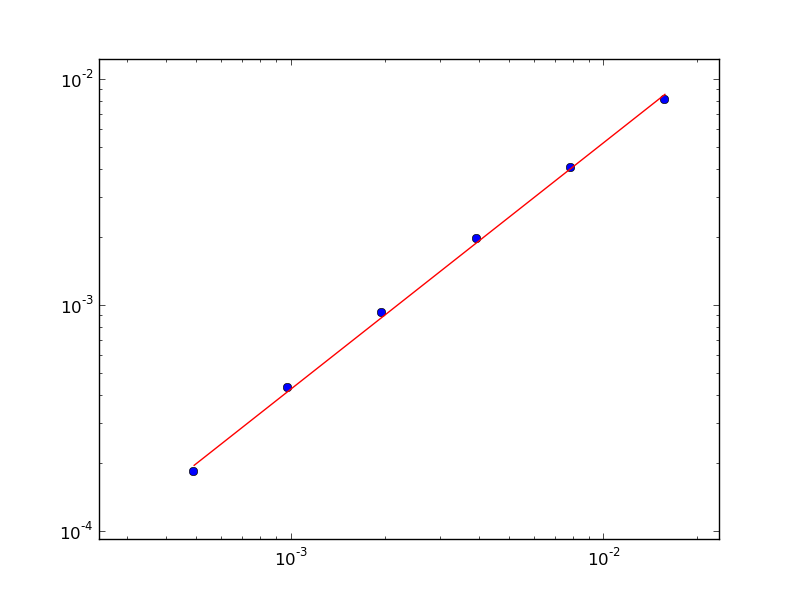
\includegraphics[width=0.5\textwidth]{loglog_error.png}\\
  \caption{Convergence of the f-wave method without limiters for smooth solutions. Plot is in loglog scale showing the $L^1$ norm of the error versus the cell length. The slope of the line is $2.0$ to two significant figures.}\label{convtest}
\end{figure}

%\section{Objective}
%\begin{enumerate}
%\item Implement the f-wave method for nonlinear elastic waves in heterogeneous media. Reproduce some of the figures in \cite{bale2002} \cite{leveque2003} and \cite{ketcheson2012}.----Almost done.
%\item Have a more comprehensive discussion of the f-wave method and problem. Mostly on the verifications of the details of the method mentioned in the paper and textbook. p. 314 $\&$ p. 333 in the textbook. Some aspects include:
%    \begin{itemize}
%    \item The disadvantages of using cell-edge flux functions in wave-propagation algorithm metioned in \cite[p. 957]{bale2002}
%    \item Justification of the Riemann solver used in \cite[p. 967]{bale2002}  ---done
%    \item The non-conservation when using w-wave in wave-propagation algorithm for 1) nonlinear autonomous systems with simple Riemann solver (HLL? p. 328 in the textbook), 2) non-autonomous systems with "Roe average" Rieman solver.    ----partially done
%    \item The non-conservation when using w-wave in wave-propagation algorithm and possible fix approximate Riemann solvers for 1) nonlinear autonomous systems with simple Riemann solver (HLL? p. 328 in the textbook), 2) non-autonomous systems with "Roe average" Rieman solver. p. 318 in the textbook
%    \item The slight difference of using $\mathcal{{\cal Z}}=s\mathcal{{\cal W}}$ in the limiter to get high-resolution methods. \cite[p. 964]{bale2002} p. 335 in the textbook.
%    \item The new line of discontinuities caused by the discontinuities of the coefficient. \cite[p. 960]{bale2002}   ---done
%    \item The breakdown of f-wave method in the case of singular flux (delta distribution).  \cite[p. 961]{bale2002}
%    \end{itemize}
%\item If possible, have some discussion on the dispersive properties of layered media i.e, solitons and shocks.
%\end{enumerate}
%The importance of the goals is decreasing in the order.
\section{Some other theoretical issues}
\subsection{Approximate Riemann solver for nonlinear elastic waves}
Since we are dealing with a nonlinear system, exact solutions to the Riemann problem is usually costly, the implementation of an approximate Riemann solver is inevitable. However, it is often enough to give good approximations as we shall see later in the numerical simulations. Here we use the approximate Riemann solver introduced in \cite{leveque2003}. For the system of conservation laws \eqref{strain} \eqref{n2}, the flux is
\begin{align}
f(q,x)=\left(
                     \begin{array}{cc}
                       -\frac{\rho(x)u}{\rho(x)}, & -\sigma(\epsilon,x) \\
                     \end{array}
                   \right)^T
\end{align}
with the Jacobian
\begin{align}
f_q(q,x)=\left(
                     \begin{array}{cc}
                       0  &  -\frac{1}{\rho}\\
                       -\sigma_{\epsilon}(\epsilon,x) &  0 \\
                     \end{array}
                   \right).
\end{align}
The eigenvalues of the Jacobian are $\pm c(q,x)$, where the wave speed is given by
\begin{align}
c(q,x)=\sqrt{\frac{\sigma_{\epsilon}(\epsilon,x)}{\rho(x)}}
\label{sounds}
\end{align}
and the corresponding eigenvectors are
\begin{align}
r^1(q,x)=\left(
                     \begin{array}{c}
                       1 \\
                       Z(q,x)
                     \end{array}
                   \right)  ,\,\,\, \mbox{for } s^1(q,x)=-c(q,x)
\end{align}
and
\begin{align}
r^2(q,x)=\left(
                     \begin{array}{c}
                       1 \\
                       -Z(q,x)
                     \end{array}
                   \right)  ,\,\,\, \mbox{for } s^2(q,x)=c(q,x)
\end{align}
where $Z(q,x)=\rho(x)c(q,x)$ is the impedance.
Instead of giving the approximate Jacobian $A_{i-1/2}$ directly, we specify the eigenvalues and eigenvectors of $A_{i-1/2}$:
\begin{align}
r^1_{i-1/2}=r^1_{i-1}=\left[
                        \begin{array}{c}
                          1 \\ Z_{i-1} \\
                        \end{array}
                      \right], & \,\,\, s^1_{i-1/2}=-\sqrt{\frac{\sigma'_{i-1}(\epsilon_{i-1})}{\rho_{i-1}}}\\
r^2_{i-1/2}=r^2_{i}=\left[
                        \begin{array}{c}
                          1 \\ -Z_{i} \\
                        \end{array}
                      \right], &\,\,\, s^2_{i-1/2}=-\sqrt{\frac{\sigma'_{i}(\epsilon_{i})}{\rho_{i}}}
\end{align}
Here we are using the solution to the eigenvalue problem of the exact Jacobian but evaluating the eigenvalues and eigenvectors according to the cells where they are. This follows from the fact that there can be no transonic rarefaction waves for these equations. As we can see from \eqref{sounds}, the existence of sonic point requires $c(q,x)=0$ which means $\sigma_{\epsilon}=0$ and the system is not hyperbolic any more. %This is the condition for creep in viscoelasitic material and will not happen in the elastic material discussed here.
One issue about using this approximate Riemann solver in the standard wave propagation form is that the "Roe condition":
\begin{align}
A_{i-1/2}(Q_i-Q_{i-1})=f_{i}(Q_i)-f_{i-1}(Q_{i-1})
\end{align}
is not satisfied.
A quick verification can be seen by checking whether ${\cal Z}^1_{i-1/2}=\beta^1 r^1=s^1_{i-1/2} \alpha^1r^1=s^1_{i-1/2}{\cal W}^1_{i-1/2}$. After decomposition,
\[
\beta^1_{i-1/2}=\frac{\sigma_i-\sigma_{i-1}+{ Z}_i(u_i-u_{i-1})}{{ Z}_i+{ Z}_{i-1}}
\]
while
\[
\alpha^1_{i-1/2}=\frac{\rho_i u_i-\rho_{i-1}u_{i-1}+Z_i(\epsilon_i-\epsilon_{i-1})}{Z_i+Z_{i-1}}
\]
with $s^1_{i-1/2}=-\sqrt{\frac{\sigma'_{i-1}(\epsilon_{i-1})}{\rho_{i-1}}}$
and $Z_i=\sqrt{\sigma'_{i}(\epsilon_{i})\rho_{i}}$. Calculation can be done to show that $ \beta^1 \neq s^1_{i-1/2} \alpha^1$. The direct consequence with the breakdown of the "Roe condition" is that the standard w-wave propagation scheme may not be conservative any more. However, it is straightforward to see that in the f-wave method, since we are decomposing $f_{i}(Q_i)-f_{i-1}(Q_{i-1})$ into waves, the flux difference will not change and be equal to the fluctuations which assembles the waves. As a result, the f-wave method allows the schemes to be conservative even if the "Roe condition" is not satisfied and it provides us more flexibility in choosing approximate Riemann solvers. On the other hand, if the Roe solver is used, in the unlimited case, the f-wave method will have exactly the same results as the standard w-wave method. In the case with limiters, the correction term in the f-wave method is
\begin{align}
\tilde{F}_{i-1/2}=\frac{1}{2}\sum_{p=1}^{m} sgn(s_{i-1/2}^{p})(1-\frac{\Delta t}{\Delta x}\abs{s^p_{i-1/2}}){\cal Z}^p_{i-1/2} \phi(\theta^p_{i-1/2}),
\label{flimiter}
\end{align}
where $\phi$ is the limiter function and $\theta^p_{i-1/2}=\beta^p_{I-1/2}/\beta^p_{i-1/2}$ is the ratio of the flux difference of the pth wave at the interface on the upwind side of $x_{i-1/2}$ over the flux difference of the pth wave at $x_{i-1/2}$. When Roe solver is used, the correction term in the w-wave method is
\begin{align}
\tilde{F}_{i-1/2}=\frac{1}{2}\sum_{p=1}^{m} sgn(s_{i-1/2}^{p})(1-\frac{\Delta t}{\Delta x}\abs{s^p_{i-1/2}})\abs{s_{i-1/2}^p}{\cal W}^p_{i-1/2} \phi(\kappa^p_{i-1/2}),
\end{align}
where
\[
\kappa^p_{i-1/2}=\frac{\alpha^p_{I-1/2}}{\alpha^p_{i-1/2}}
\neq
\frac{s^p_{I-1/2}\alpha^p_{I-1/2}}{s^p_{i-1/2}\alpha^p_{i-1/2}}
=\frac{\beta^p_{I-1/2}}{\beta^p_{i-1/2}}=\theta^p_{i-1/2}.
\]

\subsection{Discretization of flux function}
	For spatially varying flux function, flux function $f(q,x)$ can be discretized with respect to $x$ in some manner consistent with a finite-volume interpretation. In this project, we are considering cell-centered flux functions $f_i(q)$ which holds throughout the $i$th cell. For sufficiently smooth $f$, this flux function might be defined simply by $f_i(q)=f(q,x_i)$. When cell-centered flux functions are used, the generalized Riemann problem at cell interface $x_{i-1/2}$ consists of the equation
	\[
	q_t + F_{i-1/2}(q,x)_x=0
	\]
	together with the initial data, where
	\[
	F_{i-1/2}(q,x)=\begin{cases}f_{i-1}(q) & \text{if } x<x_{i-1/2}\\
	f_i(q) & \text{if } x>x_{i-1/2}\end{cases}
	\]
	It is also natural to instead assume that $f_{i-1/2}(q)$ is specified at each cell interface. This cell-edge flux functions measure the flow between cell $i-1$ and cell $i$ which is used in flux-differencing algorithm. However, when we include high-resolution corrections, and apply flux limiter, it can be interpreted as applying the limiter functions to the waves propagation form resulting from the Riemann solutions.\\
	
	\noindent The wave propagation form for cell-edge flux functions can be related to the cell-centered flux approach by viewing the flux $f_{i-1/2}(q)$ as holding over the interval $[x_{i-1},x_i]$. But that would cause discontinuity in flux at the cell centers $x_i$. The wave propagation algorithm is based on solving Riemann problem at each interface of discontinuity. For our Riemann problem at $x_{i-1/2}$, we need to solve equations $q_t+f_{i-1/2}(q)_x=0$. Also there is a jump of flux at each cell center $x_i$, which requires to consider a second set of Riemann problems. Nontrivial waves can arise from these points because of the jump in flux. And as a result, we need to include flow generated from these discontinuities.
\subsection{Breakdown of f-wave method}
The primary advantage of the f-wave method is based on that the entire flux difference is decomposed and carried by these propagating f-waves. Thus the flux is continuous across $x_{i-1/2}$. However, this is true only for conservation laws that have bounded solutions for which the flux is continuous everywhere. In one space dimension, the pressureless gas equation system is not strictly hyperbolic. The general solution for Riemann problem with constant initial value and a single discontinuity ($u_{i-1}>u_{i}$) will form delta shocks in both mass and momentum moving at constant velocity. The meaningful single valued weak solution is derived by taking pressure term goes to $0$, which gives a hyperbolic system, but also will introduce two waves with large amplitude and opposite sign. That corresponds to a jump from $Q_{i-1}$ to delta shock intermediate value, and another jump back down to $Q_{i}$. The problem with using f-wave approach is that the decomposed flux in the correction term is large enough to cause poor results. Instead, the f-wave should be considered as one single propagating wave with moving velocity equal to delta shock.
	
\section{Numerical simulation}
\subsection{Effect of impedance}
For the advective linear acoustic equations, the the reflection waves appear if and only if the impedances do not match on the two sides of the interface. Here we use the generalized Riemann problem to study the effect of impedance in the conservative form in which we show that the impedance may not be the unique quantity for the determination unless one uses another formulation. Consider the generalize Rimann problem for the linearization of Equation \eqref{strain} \eqref{n2}. i.e., for small amplitude waves with \eqref{lins} as the constitutive relation.
\begin{align}
\left(
  \begin{array}{c}
    \epsilon \\
    \rho u \\
  \end{array}
\right)_t+
\left(
             \begin{array}{c}
                      -u \\
                      -K\epsilon \\
                    \end{array}
             \right)_x=0
\end{align}
where $x=0$ is the interface of the two material,
\begin{align}
	\rho(x)=\begin{cases}\rho_l & \text{if } x<0 \\
	\rho_r & \text{if } x>0\end{cases}, \,\,\,
	K(x)=\begin{cases}K_l & \text{if } x<0 \\
	K_r & \text{if } x>0\end{cases}
\end{align}
with the initial condition
\begin{align}
	\epsilon(x,0)=\begin{cases}\epsilon_l & \text{if } x<0 \\
	\epsilon_r & \text{if } x>0\end{cases}, \,\,\,
	u(x,0)=\begin{cases}u_l & \text{if } x<0 \\
	u_r & \text{if } x>0\end{cases}
\end{align}
Let $q=(\epsilon,\rho u)^T$. The solution to the Riemann problem will consist of four states $q_l,q_l^*,q_r^*,q_r$. from the left to the right. Using the Rankine Hugoniot condition, the jump between $q_l,q_l^*$ is proportional to the left going wave in the left medium
\begin{align}
q_l^*-q_l=\alpha_1 r^1_l=\alpha_1   \left( \begin{array}{c}
                      1 \\
                      Z_l \\
                    \end{array}\right).
\end{align}
The jump between $q_r^*,q_r$ is proportional to the right going wave in the right medium
\begin{align}
q_r-q_r^*=\alpha_2 r^2_r=\alpha_2   \left( \begin{array}{c}
                      1 \\
                      -Z_r \\
                    \end{array}\right).
\end{align}
The jump between $q_l^*,q_r^*$ is determined by the continuity of the flux
\begin{align}
f_l(q_l^*)=f_r(q_r^*).
\end{align}
These equations form a linear system and we can then solve for $\alpha_1$ and $\alpha_2$ in terms of $q_l$ and $q_r$. If we follow the same assumption in the textbook that the coming wave from the left determines the generalized Riemann problem with the initial condition:
\begin{align}
q_r-q_l=\beta r^2_l=\beta\left( \begin{array}{c}
                      1 \\
                      -Z_l \\
                    \end{array}\right)
\end{align}
and the impedance matched $Z_l=Z_r=Z$
we get
\begin{align}
\alpha_1=  \frac {Z c_r (q_l)_1 -Z c_l (q_l)_1 + c_r (q_l)_2 - c_l (q_l)_2 }{2 Z c_l}\\
\alpha_2=  \beta+\frac {Z c_r (q_l)_1 -Z c_l (q_l)_1 + c_l (q_l)_2 - c_r (q_l)_2 }{2 Z c_r}
\end{align}
A wave independent of $\beta$ will be reflecting from the interface even if the impedance matches unless furthermore we assume $q_l$ or $q_r$ vanishes. However, if we consider an initial condition given by discontinuities in terms of a right-going f-wave at the interface:
\begin{align}
f_r(q_r)-f_l(q_l)={\cal Z}^2=\beta \left( \begin{array}{c}
                      1 \\
                      -Z_l \\
                    \end{array}\right)
\end{align}
then we get the coefficients for the f-waves for the solution to the generalized Riemann problem:
\begin{align}
\alpha_1= {\frac { {\it Z_r}-{\it Z_l}
  }{{\it Z_l}+{\it Z_r}}}\beta\\
\alpha_2=  \frac {{2}\,{\it Z_l}\,}{ {\it Z_l}+{\it Z_r}  }\beta.
\end{align}
in which case the impedance is the only factor for the reflection wave. This again implies that thinking in terms of the f-wave is a better and may possibly be a more fundamental idea of the wave-propagation method.
Figure \ref{imp} shows a stress wave passing through the interface of two homogeneous nonlinear materials. In the plots on the left column, the two materials have the same impedance and the same sound speed, we see the wave is sharpening in the front and is followed by a rarefaction wave due to the nonlinearity. In the plots in the middle column, the stress wave is passing through the interface but the shape changes not only due to the nonlinearity but also because of the sound speed change in the material. In the plots on the right column, instead of the generation of the shock from the nonlinear effect, part of the wave is bouncing back when the wave hits the interface while the rest passes through the interface. From here, we could imagine that in the periodic layered media, the waves will be constantly bouncing back between the interfaces. As a result, this gives rise to an equivalent dispersion effect.
\begin{figure}
  % Requires \usepackage{graphicx}
  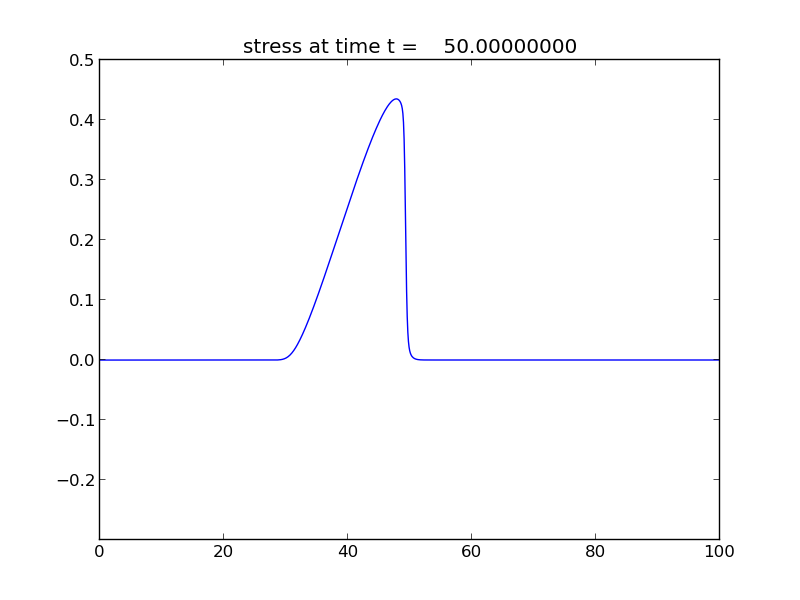
\includegraphics[width=0.3\textwidth]{homo1.png}
  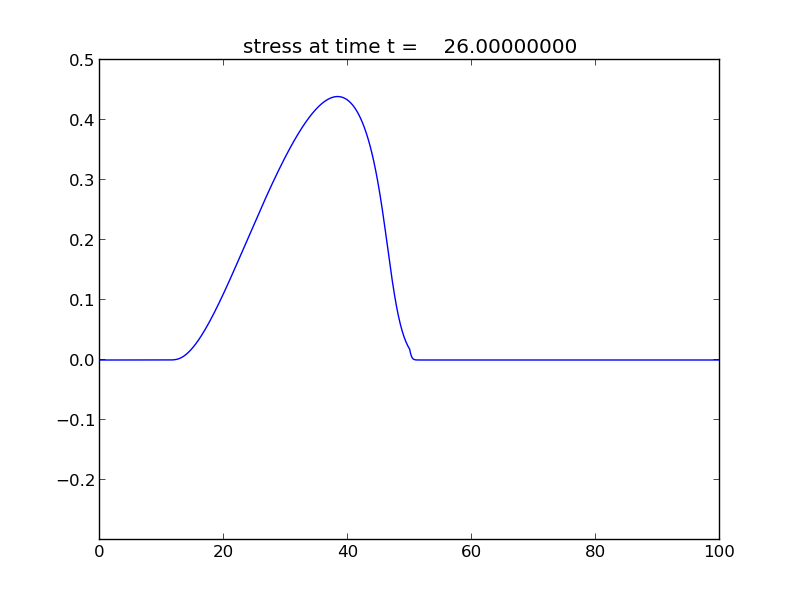
\includegraphics[width=0.3\textwidth]{sound1.png}
  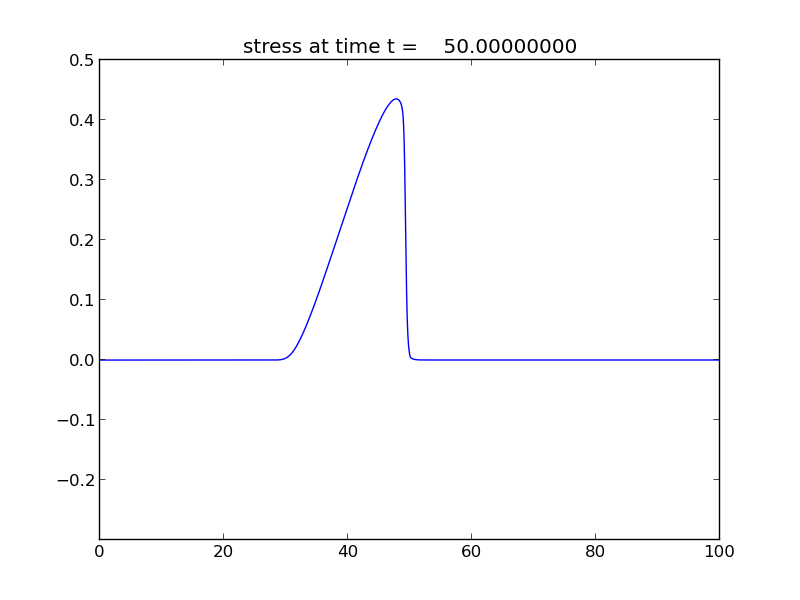
\includegraphics[width=0.3\textwidth]{reflect1.png}\\
  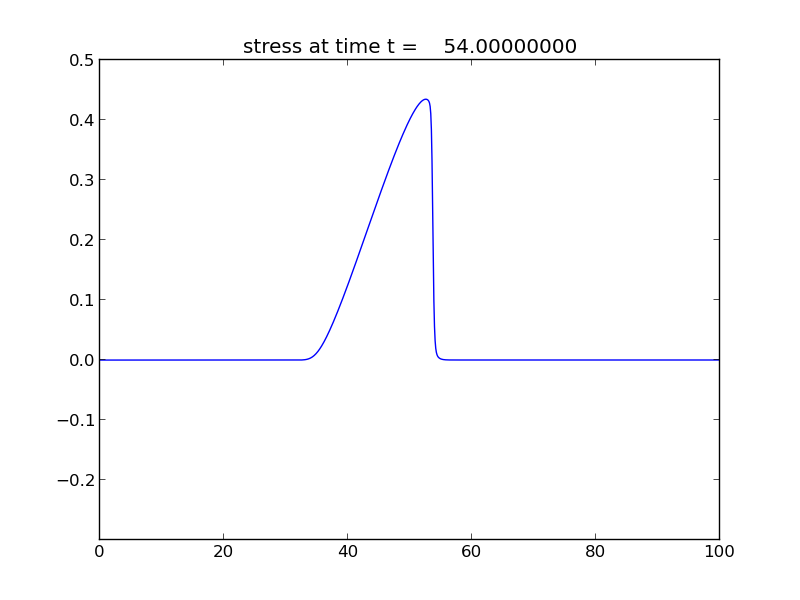
\includegraphics[width=0.3\textwidth]{homo2.png}
  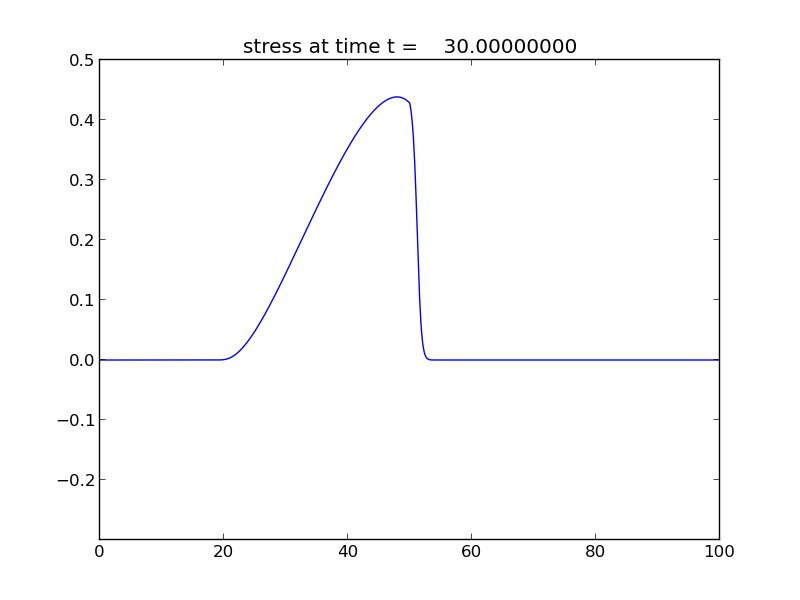
\includegraphics[width=0.3\textwidth]{sound2.png}
  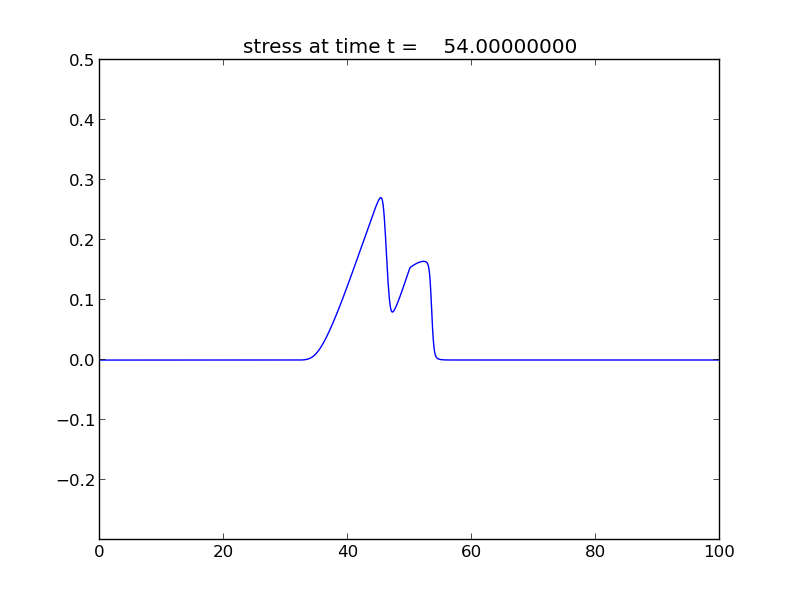
\includegraphics[width=0.3\textwidth]{reflect2.png}\\
  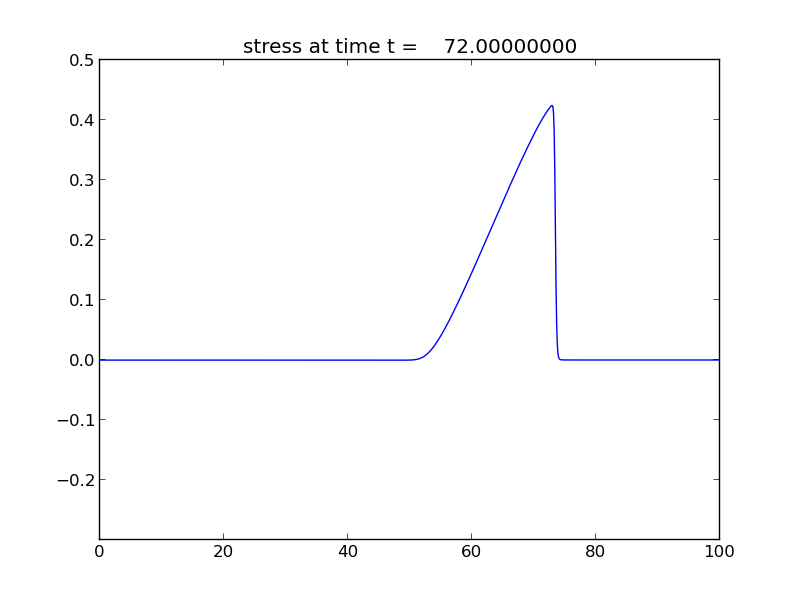
\includegraphics[width=0.3\textwidth]{homo3.png}
  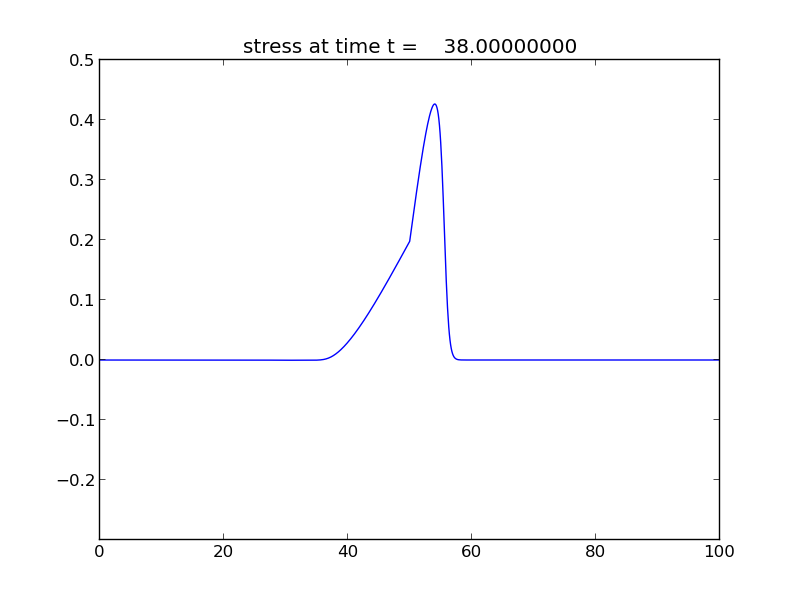
\includegraphics[width=0.3\textwidth]{sound3.png}
  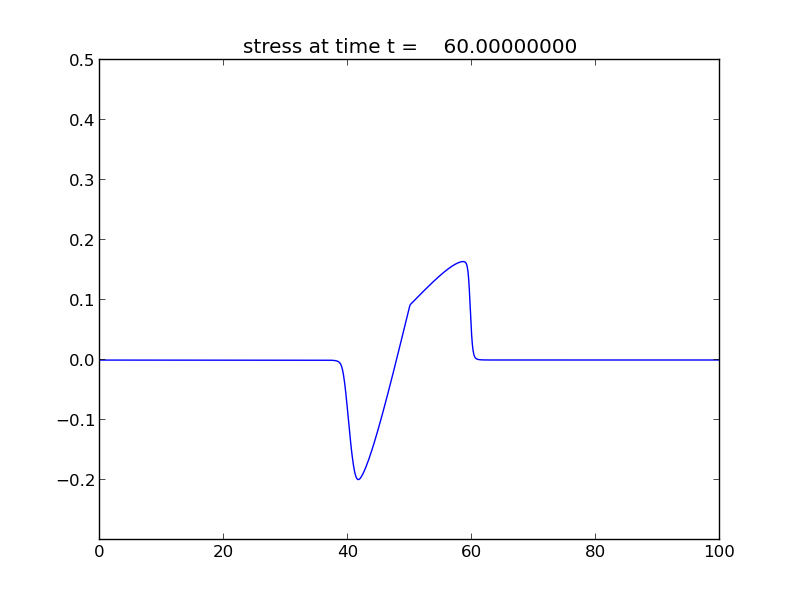
\includegraphics[width=0.3\textwidth]{reflect3.png}\\
    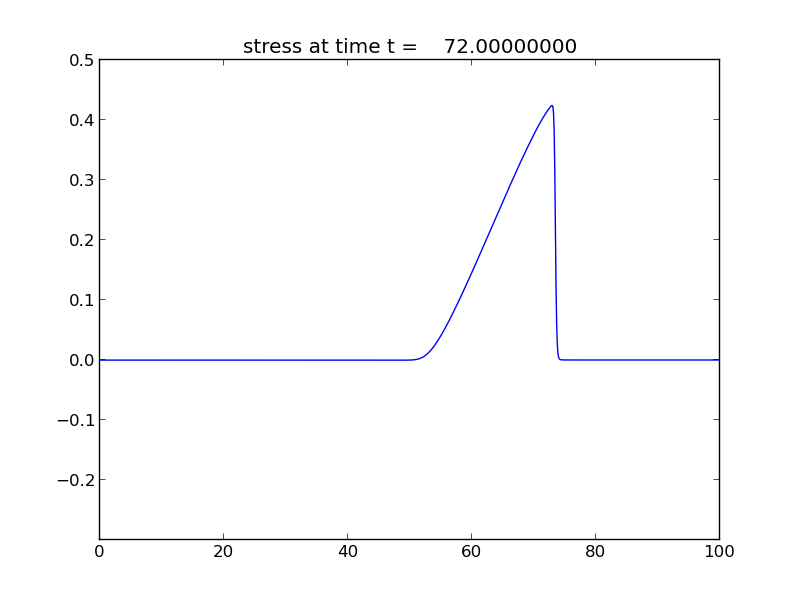
\includegraphics[width=0.3\textwidth]{homo4.png}
  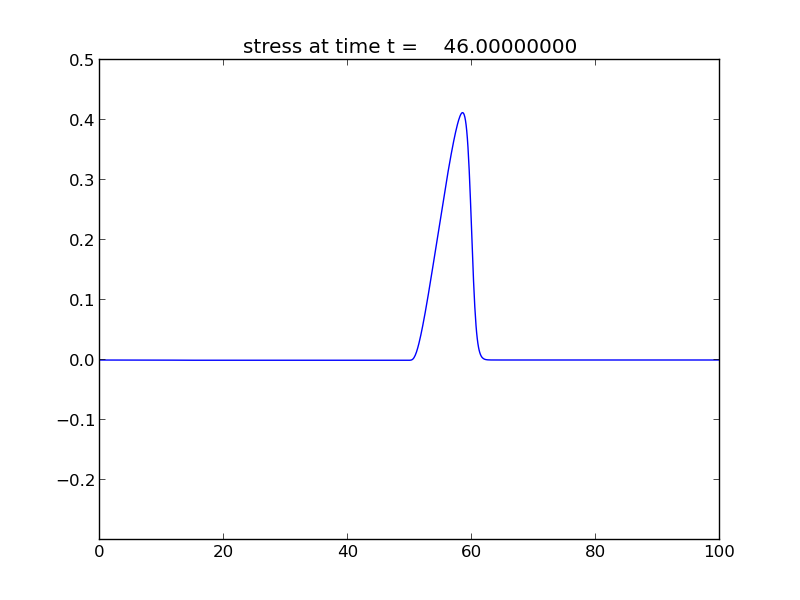
\includegraphics[width=0.3\textwidth]{sound4.png}
  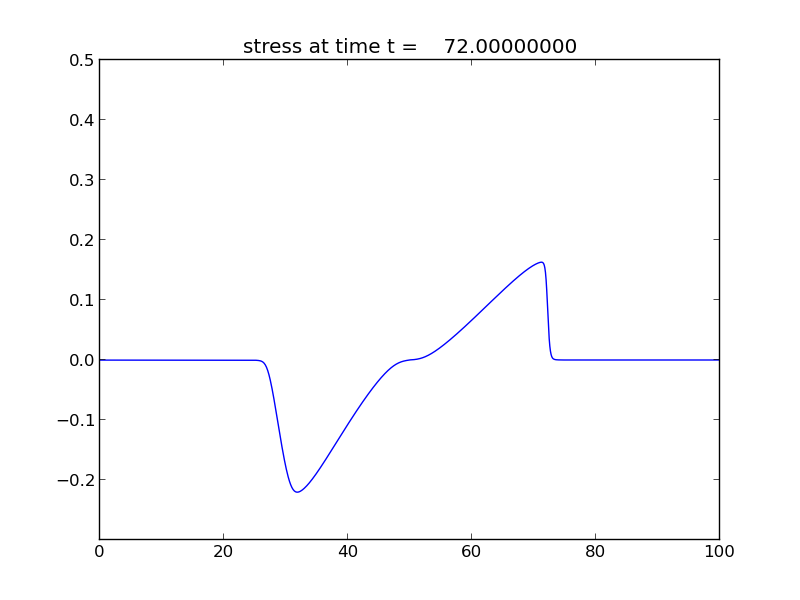
\includegraphics[width=0.3\textwidth]{reflect4.png}
  \caption{The wave travelling through the interface (at $x=50$) of two materials. Left column: two homogeneous materials with the same impedance and sound speed. Middle column: two homogeneous materials with the same impedance and different sound speeds. Right column: two homogeneous materials with different impedances and the same sound speed.}
  \label{imp}
\end{figure}

\subsection{Dispersion and stegotons}
Using the homogenized equations for the layered media discussed in the textbook, as shown in \cite{leveque2003} we can study the asymptotics for the averaged solutions over many layers. Without getting into the details. we only include the conclusion that along with a constant coefficient acoustic equation, there will be an extra third order spatial derivative in the homogenized equation. This introduces dispersions like in the KdV equation. Therefore, we hope the dispersion will interact with the nonlinearity and produce soliton solutions for the periodic layered media. This is indeed true. In Figure \ref{travelw}, an initial smooth cosine strain wave is coming from the left boundary. As time goes on, four soliton-like solutions come out of the single wave. However, the soliton-like waves actually contains several stationary contact discontinuities and do not have a fixed profile. Since they look like the back of the Stegosaurus, they are named stegotons. We take a close look at the waves in Figure \ref{collision} and simulate the collision of two stegotons. They seem to have similar behavior as the usual solitions in KdV equations. The shapes of the stegotons are approximately maintained after the collision following by some small wave packets.

\begin{figure}
  % Requires \usepackage{graphicx}
  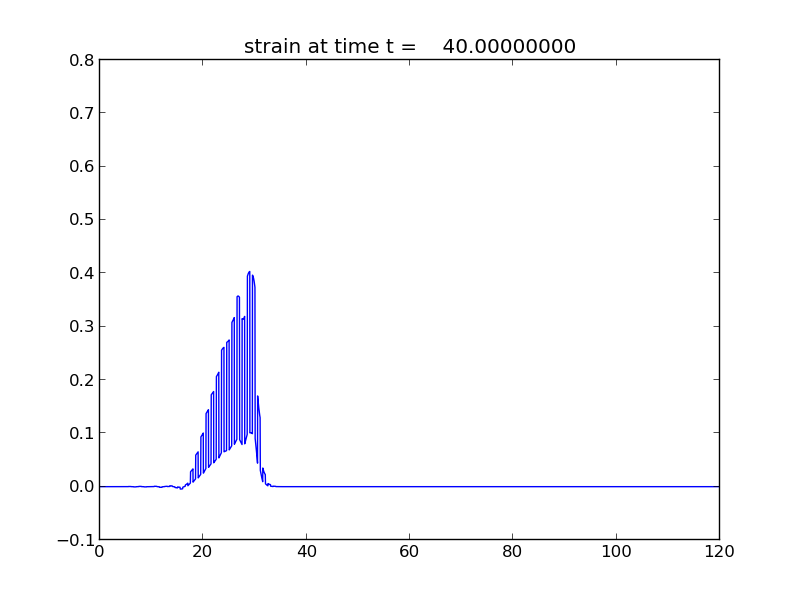
\includegraphics[width=0.5\textwidth]{frame0004fig1.png}
  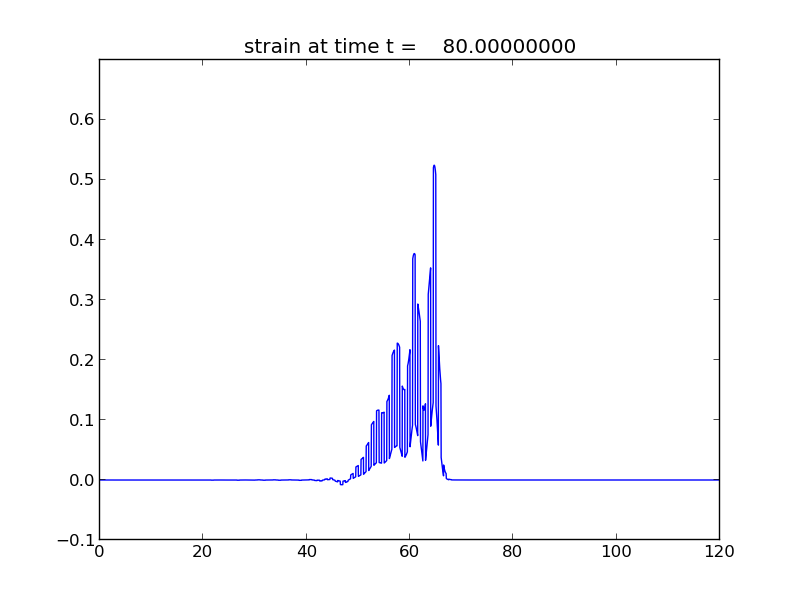
\includegraphics[width=0.5\textwidth]{frame0008fig1.png}
  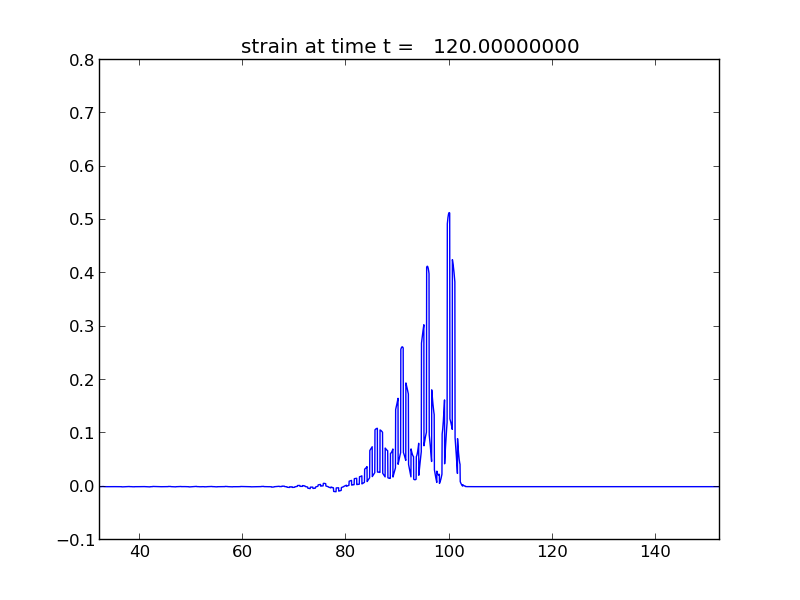
\includegraphics[width=0.5\textwidth]{frame0012fig1.png}
  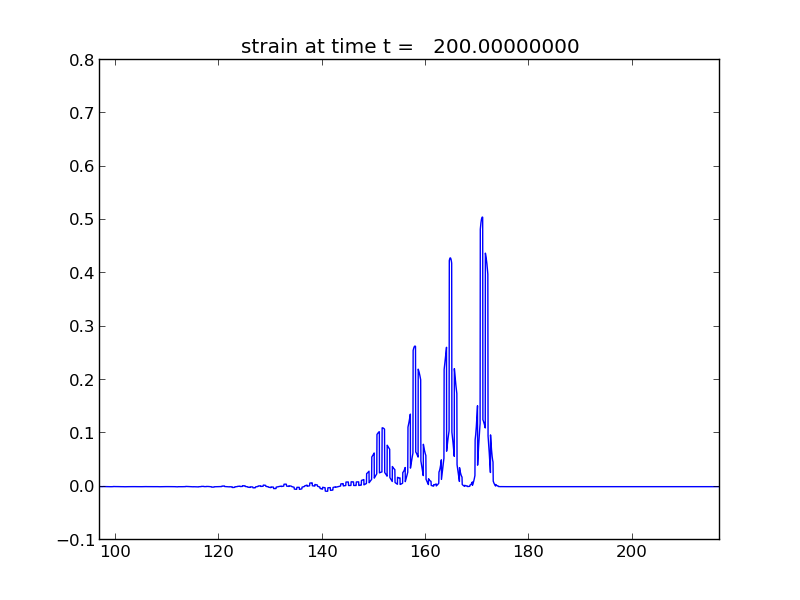
\includegraphics[width=0.5\textwidth]{frame0020fig1.png}
  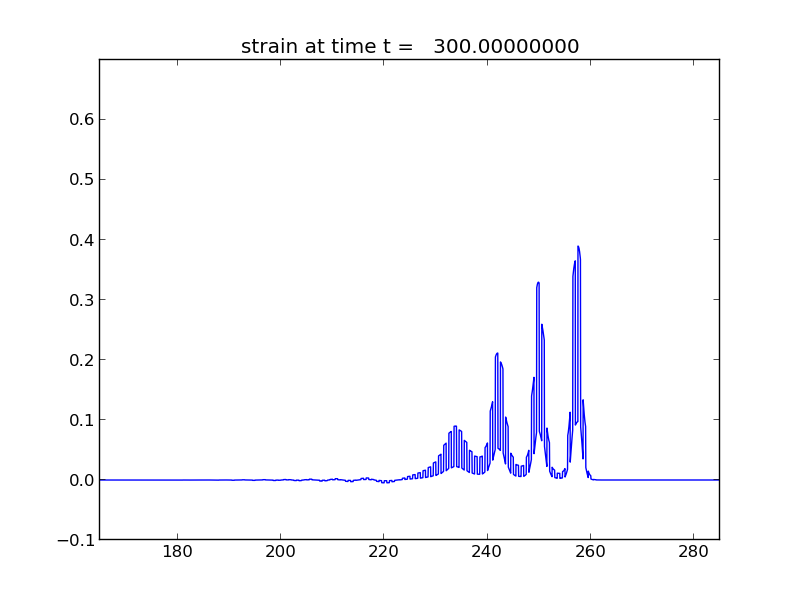
\includegraphics[width=0.5\textwidth]{frame0030fig1.png}
  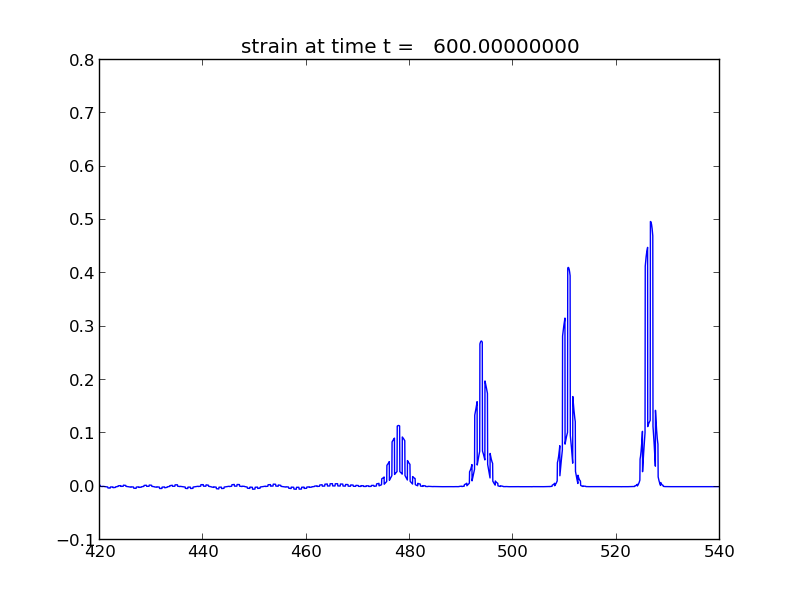
\includegraphics[width=0.5\textwidth]{frame0060fig1.png}
  \caption{The decomposition of the initial single bump into soliton-like waves.}
  \label{travelw}
\end{figure}

\begin{figure}
  % Requires \usepackage{graphicx}
  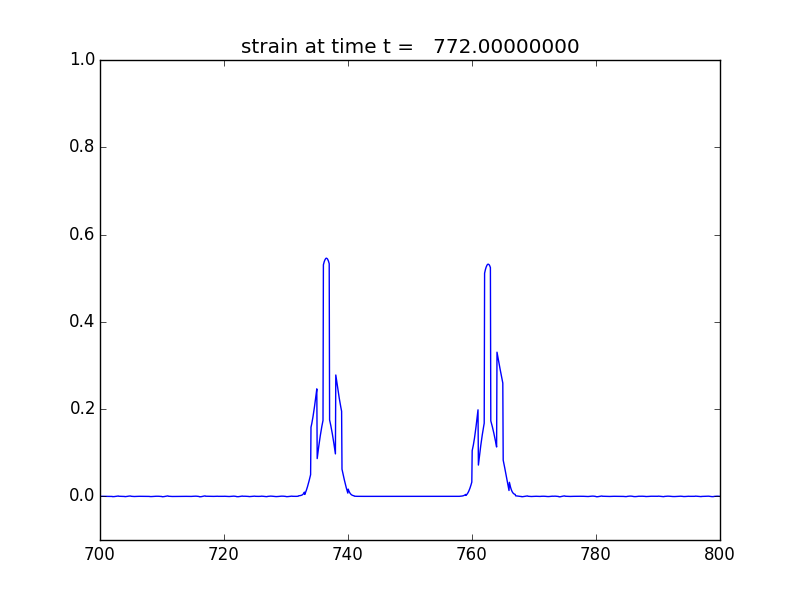
\includegraphics[width=0.4\textwidth]{stegoton1.png}
  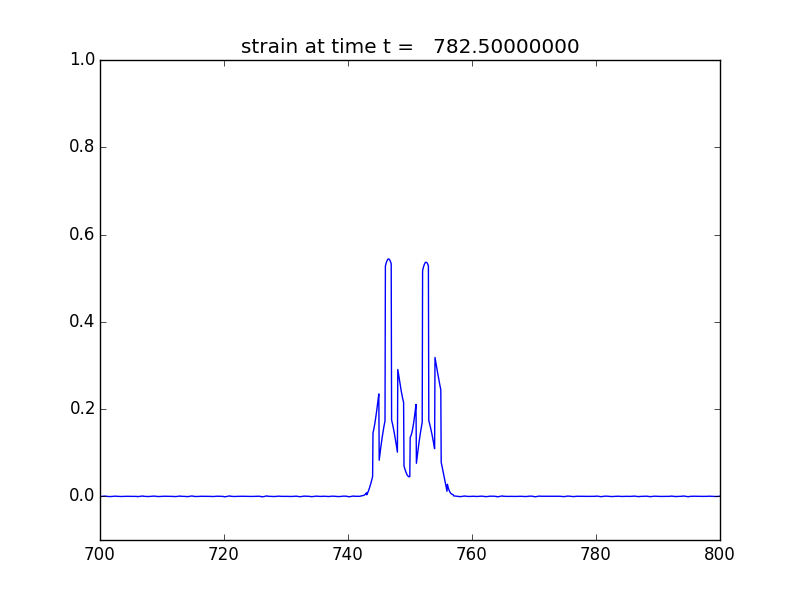
\includegraphics[width=0.4\textwidth]{stegoton2.png}\\
  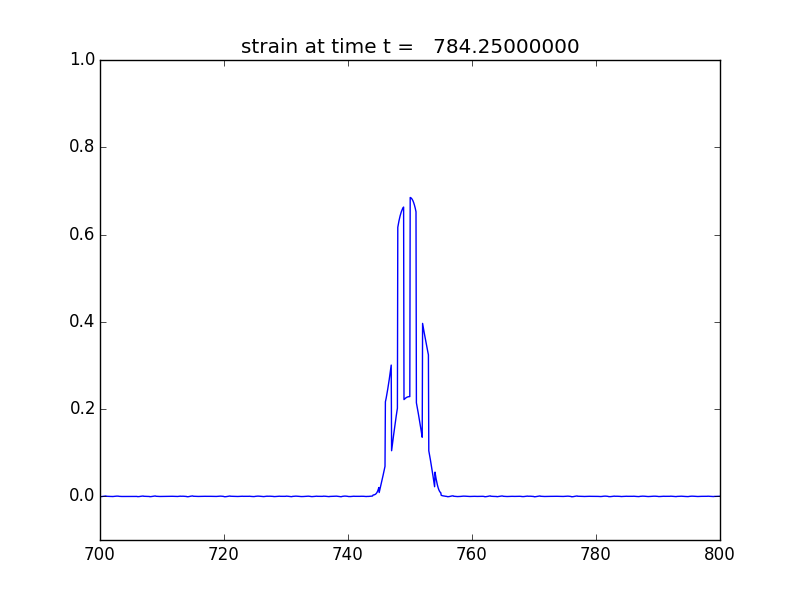
\includegraphics[width=0.4\textwidth]{stegoton3.png}
  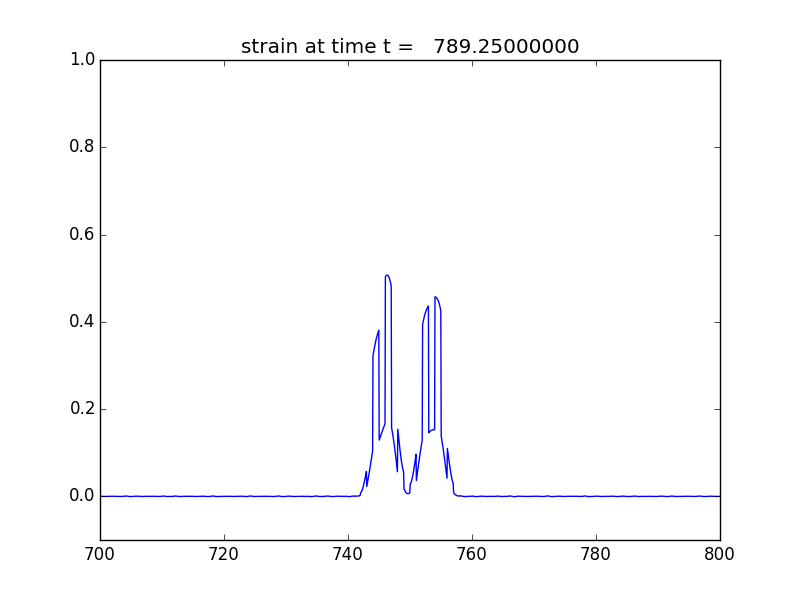
\includegraphics[width=0.4\textwidth]{stegoton4.png}
  \caption{The collision of two stegotons.}
  \label{collision}
\end{figure}


\section{Summary}
In this project, we show that in the case where the flux is spatially variable, the f-wave method is a better formulation for solving hyperbolic conservation laws using wave-propagation form. It is better and more convenient to use f-wave method since the method allows Riemann solver to maintain conservation even if the Roe condition is not satisfies and avoids the implementation of the extra discontinuities from the variable coefficients. In the numerical simulations for nonlinear layered media, we see that in the case where the impedance of the layered media is not constant, the f-wave will reflect when it hits the interface. The constant reflection finally gives rise to an equivalent dispersion which combines the nonlinearity and produces solutions look like and behave similar to solitons.
%\section{Appendix A: MATLAB functions used and brief implementation explanation}
%\section{Appendix B: MATLAB codes}
%\section{Appendix C(optional)} Any algebraically intense calculations.

\begin{thebibliography}{9}
\bibitem{bale2002}
D. S. Bale, R. J. LeVeque, S. Mitran, and J. A. Rossmanith, SIAM J. Sci. Comput 24 (2002), 955-978.
\bibitem{leveque2002}
Finite Volume Methods for Nonlinear Elasticity in Heterogeneous Media
by R. J. LeVeque, Int. J. Numer. Meth. Fluids 40 (2002), pp. 93-104.
\bibitem{leveque2003}
Randall J. LeVeque and Darryl H. Yong, SIAM J. Appl. Math., 63 (2003), pp. 1539-1560.
\bibitem{ketcheson2012}
David I Ketcheson, Randall J. LeVeque Comm. Math. Sci. 10 (2012), pp. 859-874.

\end{thebibliography}

\end{document}
